\documentclass[a4paper]{article}

\usepackage{color}
\usepackage{url}
\usepackage[T2A]{fontenc} % enable Cyrillic fonts
\usepackage[utf8]{inputenc} % make weird characters work
\usepackage{graphicx}

\usepackage[english,serbian]{babel}
%\usepackage[english,serbianc]{babel} %ukljuciti babel sa ovim opcijama, umesto gornjim, ukoliko se koristi cirilica

\usepackage[unicode]{hyperref}
\hypersetup{colorlinks,citecolor=green,filecolor=green,linkcolor=blue,urlcolor=blue}

%\newtheorem{primer}{Пример}[section] %ćirilični primer
\newtheorem{primer}{Primer}[section]

\begin{document}

\title{Stiven Hoking\\ \small{Seminarski rad u okviru kursa\\Tehničko i naučno pisanje\\ Matematički fakultet}}

\author{Lazar Rajčić\\ lazarrajcic23@gmail.com}
\date{14.~novembar 2022.}
\maketitle

\abstract{
Razlog zašto smo izabrali da pišemo o Stivenu Hoking-u jeste da bi ljudima približili njegove doprinose nauci uprkos barijerama koje je predstavljala njegova bolest. Unutar ovog seminarskog smo ispričali kratko njegovu životnu priču i objasnili neke od njegovih teorija.  

\tableofcontents

\newpage

\section{Uvod}
\label{sec:uvod}
Pre nego sto počnemo sa pričom o životu Stivena Hokinga i njegovim dostignućima moramo napraviti mali uvod u to ko je zapravo Stiven Hoking.
Stiven Hoking je bio engleski teoretski fizičar i kozmolog. Zbog njegovih doprinosa fizici smatran je za jednog od najvecih naučnika svog vremena. Njegovi doprinosi fizici se uglavnom nalaze u domenu našeg poznavanja crnih rupa ali o tome ćemo detaljnije pisati u zaglavlju Karijera. Zbog ovoga smatramo da je jako važno približiti njegova dostignuća ljudima.
Tematika ovog seminarskog rada je život i dostignuća Stivena Hokinga. Manja zaglavlja seminarskog su: Život, koji se dalje deli na život pre i posle dijagnoze, i Karijera.

\section{Život}
\subsection{Život pre dijagnoze i dijagnoza (rani život)}
Hoking se rodio 8. Januara 1942. Godine, tačno na tristotu godišnjicu smrti njegove 
velike inspiracije Galilea Galileja. Iako iznenđujuće nije bio najbolji ucenik, 
Stivena je od ranih nogu izuzetno interesovalo kako univerzum funkcioniše. Čak će u 
kasnijim godinama reći da ako razumemo kako univerzum radi mozemo u neku ruku i da ga 
kontrolišemo. Ova znatiželja koja će ga kasnije u životu gurati u napredovanju kariere,
u školi mu je zaslužila nadimak Ajnštajn. Planovi za dalje studiranje matematike 
ometeni su od strane njegovog oca koji je smatrao da u tome nema budućnosti. Usledio 
je kompromis, kojim je odlučeno da će Stiven da pohađa osnovne studije na polju fizike
na Oksfordu. Osnovne studije je zavrsio 1962. godine sa diplomom prvog reda posle 
čega se uputio na dalje obrazovanje na Kembridž univerzitetu. \medskip

Pri početku svojih studija na Kembridž-u Stiven je primetio da nesto nije sasvim u 
redu. Postao je vise trapav i imao je poteskoce sa malim stvarima poput vezivanja 
pertli. Nakon incidenta na klizanju majka ga je odvela u bolnicu na testiranje. Ne 
dugo nakon njegovog 21-og rodjendana saznaje se da ima neizlečivu bolest. Ta bolest 
se ispostavilo da je amiotrofička lateralna skleroza (eng. Amyotrophic lateral 
sclerosis) skraćeno ALS. To je bolest koja napada motorne nerve i polako ih uništava, 
ali nema efekta na mozak. Tadašnji doktori su zaključili da neće živeti duže od još 
dve godine. Ova vest ga je očekivano demoralizovala. Medjutim ubrzo nalazi ponovnu 
inspiraciju u Vagnerovoj muzici i ljubavi prema Džejn Vajld, svojoj buducoj supruzi. 
Kako je sada imao za koga da zivi, Stiven se ponovo bacio u svoja istraživanja koja 
su mu se, na sopstveno iznenadjenje, jako dopala. 

\begin{figure}[h!]
\centering
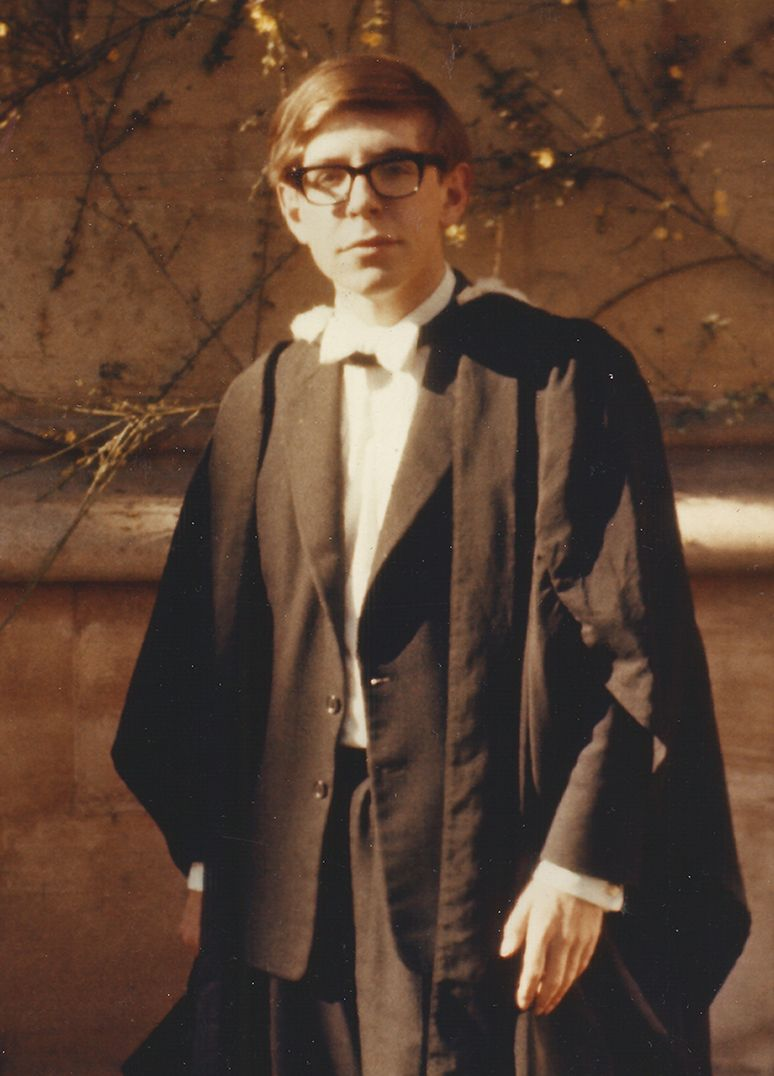
\includegraphics[width=0.5\textwidth]{Hoking,PreDijagnoze.jpg}
\caption{Hoking, na dodeli diploma 1960.}
\end{figure}

\subsection{Život nakon dijagnoze}
Iako je otpočeo karijeru sa puno entuzijazma, njen tok je bio dosta nepredvidljiv. 
Na Kembridž-u nije uspeo da nastavi studije pod Fredom Hojlom, u to doba izuzetno 
uglednim astronomom, kao sto je bila njegova zelja, jer je Hojl već imao previše 
studenata tada. Karijeru je zato otpočeo pod fizičarom i kozmologom Denisom Škiamom. 
Na ovo u kasnijim godinama Stiven gleda kao vrlo srećnu okolnost, koja je postavila 
temelje njegove dalje karijere. Govoreći takodje kako nije verovatno da bi dostigao 
veliki uspeh pod Hojlovim nadzorom. Ovo je potvrdila njihova javna prepirka 1964. 
godine, kada je Hoking prekinuo Hojlovo predavanje kako bi ukazao na grešku uglednog 
naučnika. \medskip

\end{document}
